\chapter{Helium-Neon-Laser} \label{aufbau helium neon laser}

In diesem Versuch wird der Laser sebler zusammengestellt.

Damit es überhaupt ein Laser gibt, werden drei folgende Komponenten benötigt:

Ein \textbf{Aktives Madium}, was mindestens ein Drei-Niveau-System sein muss, damit eine Besetzungsinversion hergestellt werden kann.
Eine \textbf{Optische Pumpe}, welche Energie für die notwendige Besetzungsinversion hinzuführt.
Und ein \textbf{Optischer Resonator}, was zu unterschtützung der stimmulierten Emission im Lasermedium, der Selektrion der Wellenlänge dient und die Strahlrichtung des Lasers.

Das Laserlicht hat mehrere eigewnschaften. Durch die Besetzungsinversion ist das Licht nahezu monochromatisch und stark kohärent.
Durch den Optischen Resonator, ist der Laserstrhal stakr gebündelt und erreicht dabei sehr große Intensität.

In diesem Versuch Haben Wir einen Aktives Medium aus Gas von Helium (He) und Neon (Ne) mit einen überwiegenden Anteil von Helium, ungefähr 10:1. 

\FloatBarrier
\begin{figure}[htbp]
    \centering
    \includegraphics[width=1\linewidth]{}
    \caption{Energielevel fur Helium- und Neonatome. Der Energietransfer für den Laserprozess wird schematisch dargestellt \ref{Prakticum}}
    \label{fig:He-Ne}
\end{figure}
\FloatBarrier

Die zum Betrieb notwendige Pumpenergie wird durch Helium bereitgestellt. 
Dabei werden Heliumatome mittels einer elektrischen Gasentladung in einen metastabilen angeregten Zustand überführt. 
Die Energie dieses Zustands liegt nahezu auf dem gleichen Niveau wie die des angeregten 3s$_2$-Zustands der Neonatome (siehe Abb.\ref{fig:He-Ne}), die durch inelastische Stoßprozesse eine Energieübertragung von Helium auf Neon überliefert.
Gelangen die Elektronen der Neonatome in den 3s$_2$-Zustand, ist ein Übergang über stimmulierte Emission in den 2p$_4$-Zustand möglich, wobei das Licht mit einer Wellenlänge von 632,8 nm abgesendet.
Im Anschluss daran kehren die elektronen der Neon atome über spontane Emission in den Grundstand zurück, wobei der Zyklus abgeschlossen wird und der Prozess von vorne beginen kann.
Zu bemerken ist, dass es nicht nur dieses eine Übergang gibt, es gibt zusätzliche übergänge, siehe Abb. \ref{fig:Übergang}, gibt.
Diese sind aber noch andere übergänge, z.B. im infraroten berreich, die aber durch die durch ein Schmalbandige Spiegel, eliminiert werden, da diese nur das rote Licht gut reflektiert.
\FloatBarrier
\begin{figure}[htbp]
    \centering
    \includegraphics[width=1\linewidth]{}
    \caption{Übergange im Neon atoms}
    \label{fig:Übergang}
\end{figure}


\subsection{Aufbau}


In diesem Versuch ist vorsich vorgeboten.


Dieser wird alles auf einer einzigen optischen Bank gemacht.
Es wird zualler erst das opitsche Achse eingestellt werden, dazu wird ist Zusätzliches Laser \textit{Pilotlaser} eingerichtet, um dieses so präziese  eizustellen zu können wie möglich. 
\FloatBarrier
\begin{figure}[htbp]
    \centering
    \begin{minipage}[t]{0.48\textwidth}
        \centering
        \includegraphics[width=\textwidth]{}
        \caption{A}
        \label{fig:Blende}
    \end{minipage}
    \hfill
    \begin{minipage}[t]{0.48\textwidth}
        \centering
        \includegraphics[width=\textwidth]{}
        \caption{B}
        \label{fig:Spiegel}
    \end{minipage}
    \caption{A: Justierung der Optischen Achse; B: Justierung der Resonator Spiegel \cite{praktikum}}
\end{figure}
\FloatBarrier
Dazu wird zuerst nur die Blende eingstellt, damit es eine definierte Achse gibt, siehe Abb.\ref{fig:Blende}.
Danach wird die Entladungsröhre eingebaut und so eingestellt, dass möglich wenig Licht innerhalb der Röhre verloren geht.
Zulätzt müssen beide Resonatorspiegel justiert werden, ohne der Entladungsröhre. 
Dazu wird die sphärische, so wie die halbdurchloässigen Planspiegel ohne die Entladungsröhre, justiert.  
Die Spiegel werden Schritt für Schritt so justiert, dass es keine Reflexe mehr auf der Wand sichtbar sind, siehe \ref{fig:Spiegel}.
Zulätzt, wird der Pilotlaser entfernt und die Entladungsröhre eingeschaltet. 
Es wird nun der Spiegel so justiert werden, bis der Laser aufblitzen sieht.

Der Laser ist jetzt aktiv und kann genutzt werden, um den Versuch durch zu führen. 
%===============================================================================================================================================================================================================================================================================================================================================

\chapter{Bestimmung der Wellenlänge des Helium-Neon Experimentierlasers mit einem Reflexionsgitter}

Um die Wellenlänge des Lasers zu bestimmen wird ein Gitter auserhalb des Optischen Resonators eingebaut, hinter den Halbdurchlässigen Resonator.
Dadurch kann durch den Optischen Zusammenhänge:
\begin{equation*}
    \tan(\alpha_i) = \frac{d_i}{a}
\end{equation*}
\begin{equation*}
    \sin(\alpha_i) = \frac{\delta}{g}; \qquad \text{mit} \qquad \delta = i \cdot \lambda
\end{equation*}
\begin{equation*}
    \Rightarrow \lambda = \frac{\sin\big(\arctan\big(\frac{d_i}{a}\big)\big)}{i \cdot g} \label{eq:Wellenlänge}
\end{equation*}
\begin{equation*}
    \Delta \lambda = \frac{1}{i \cdot g} \cdot \frac{1}{(d_i^2 + a^2)^\frac{3}{2}} \cdot \sqrt{(a^2 \cdot \Delta d)^2 + (da \cdot \Delta a
    )^2}
\end{equation*}
Dies lässt sich aus der Abb. \ref{fig:Gitter} herleiten.
\FloatBarrier
\begin{figure}
    \centering
    \includegraphics[width=1\linewidth]{}
    \caption{Funtion eines Gitters zzur betimmung der Wellenlänge \cite{das-optische-gitter}}
    \label{fig:Gitter}
\end{figure}
Mit der Gitterkonstante von $g = 600 \frac{\text{lines}}{mm}$ un den Werten in Tabelle \ref{tab:Wellen} können in formel \ref{eq:Wellen} eingesetzt werden.

\begin{table}[htbp]
    \centering
    \begin{tabular}{c|c|c|c}
        \text{Ordnung} & \(d_i ~[\text{m}]\) & \(a ~[\text{m}]\) & \(\lambda~[\text{nm}]\)\\
        \hline
        -1. & 0,823 \(\pm\) 0,006 & 1,964 \(\pm\) 0,006 & 644,14 \(\pm\) 4,70 \\
        1. & 0,824 \(\pm\) 0,006 & 1,964 \(\pm\) 0,006 & 644,80 \(\pm\) 4,70 \\
    \end{tabular}
    \caption{Werte der Polarisation}
    \label{tab:WPolar}
\end{table}

Die weitern Ordnungen konnten nicht bestimmt werden, da diese nicht sichtbar waren, oder da die Wand nicht breit genug war. 

Mit hilfe diese Werte kann die mittlere Wellenlänge als $\lambda = (644,47 \pm 3,32)$ nm berechnet werden.

Im vergleich mit dem Erwarteten Wellenlänge des Neon-Laserübergangs von $3s_2 \rightarrow 2p_4$ von 632,8 nm, siehe Abb. \ref{fig:He-Ne}, ist es sichtbar, dass es eine significante Abweichung gibt. 
Der Wert weicht um ca. 1.8$\%$ von dem Literaturwert ab. 
Auch mit den Fehler ist der Literaturwert nicht enthalten.
Dies Könnte an ein zu geringe abschätzung von den Fehlerwerten liegen, oder dessen Ablesen.
Es könnte auch sein, dass der Gitter nicht ganz orthogonal Ausgerichtet ist, oder dass die Wand nicht ganz orthogonal zum Laserstrahl ist und somit die Messung verfälscht werden könnte. 
Es war auch keine unsicherheit an dem Gitter für die Gitterkonstante angegeben, wodurch der Fehler größer sein könnte. 
Zusätzlich ist es sehr warscheinlich das die Spiegel, die nur das rote licht durchlassen soll, nicht das ganze andere Licht blockiert, sonder auch noch kleine anteile von anderen Wellenlängen.



%===============================================================================================================================================================================================================================================================================================================================================
\chapter{Untersuchung der Polarisation des Experimentierlasers}

Da der Laser das Licht in alle richtungen streut, wurde versucht mithilfe von Brewster-winkel, dass der Laser Polar linearisiert wird indem, dieser zum größten teils nur den Linearpolarisierten teil durch lässt und mit einer anreiheung der Brewster-fenster, so viel von dem anderen Polaristierten Lichts ablenkt. 

Um dies zu untersuchen, wird ein Polarisator eingebaut und eine langsame Photodiode, siehe (Abb. \ref{fig:Polar}.

\begin{figure}
    \centering
    \includegraphics[width=1\linewidth]{}
    \caption{Aufbau zur bestimmung der Polarisation}
    \label{fig:Polar}
\end{figure}

Es wurde für verschidene polarisation die Spannung gemessen, die durch einen 50 $ \ohm $ Widerstand den Stromfluss vergrößert hat, damit es sichtbar ist.
Die Werte sin din tablelle \ref{tab:Wellenlänge} aufgelistet.

\begin{table}[htbp]
    \centering
    \begin{tabular}{c|c}
        Winkel\(~[\text{°}]\) & U \(~[\text{mV}]\) \\
        \hline
        0 \(\pm\) 1 & 10 \(\pm\) 1,5 \\
        20 \(\pm\) 1 & 1,75 \(\pm\) 0,3 \\
        40 \(\pm\) 1 & 2 \(\pm\) 0,5 \\
        60 \(\pm\) 1 & 2,2 \(\pm\) 0,5 \\
        80 \(\pm\) 1 & 11,5 \(\pm\) 1 \\
        100 \(\pm\) 1 & 21 \(\pm\) 2 \\
        120 \(\pm\) 1 & 27,5 \(\pm\) 3 \\
        140 \(\pm\) 1 & 25 \(\pm\) 3 \\
        160 \(\pm\) 1 & 17 \(\pm\) 2 \\
        180 \(\pm\) 1 & 7,5 \(\pm\) 1 \\
        200 \(\pm\) 1 & 0,9 \(\pm\) 0,3 \\
        220 \(\pm\) 1 & 1,7 \(\pm\) 0,3 \\
        240 \(\pm\) 1 & 2,8 \(\pm\) 0,35 \\
        260 \(\pm\) 1 & 11 \(\pm\) 1 \\
        280 \(\pm\) 1 & 18 \(\pm\) 1,5 \\
        300 \(\pm\) 1 & 24 \(\pm\) 2 \\
        320 \(\pm\) 1 & 21 \(\pm\) 2 \\
        340 \(\pm\) 1 & 13 \(\pm\) 1,5 \\
    \end{tabular}
    \caption{Werte der Wellenlängen bestimmung}
    \label{tab:Wellen}
\end{table}

Da das Laser Linear polarisiert sein soll können di9e Werte durch das Malus'sche-Gesetz beschrieben werde. 
Dies besagt, dass die Polarisation von Linear Polarisiertem licht in der form von cosiuns quadrat von dem Polarisations winkel abnimmt.
\begin{equation*}
    I = I_0 \cdot \cos^2(\Theta -\Theta_0) + b
\end{equation*}
Die ausgerechnete werte sind in tabelle \ref{tab:WertePol}:

\begin{table}[htbp]
    \centering
    \begin{tabular}{c|c}
        Parameter & Wert \\
        \hline
        $U_0$ & (21.59 \(\pm\) 0.79) mV \\
        $\theta_0$ & (125.97 \(\pm\) 0.64) ° \\
        $b$ & (0.22 \(\pm\) 0.17) mV \\
    \end{tabular}
    \caption{Werte von der Polarisation}
    \label{tab:WertePol}
\end{table}

Dies lässt sich in folgende Abb. \ref{fig:PolarisationFigur} sehen.

\begin{figure}
    \centering
    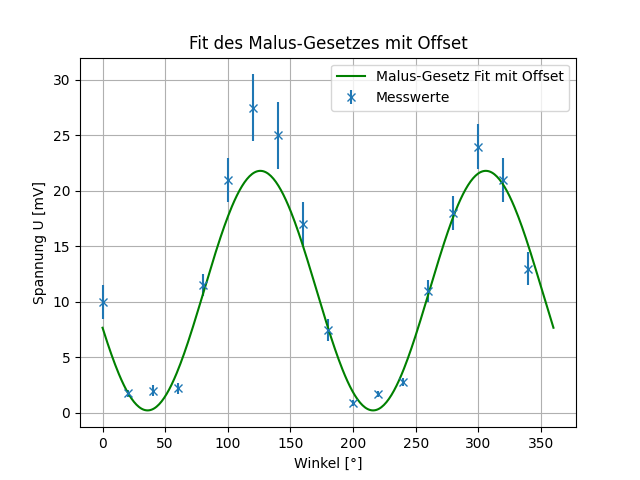
\includegraphics[width=1\linewidth]{figs\Figure_2}
    \caption{Angepasste Cosinusfunktion mit den Werten $\chi^2_{red} = 5.16$}
    \label{fig:PolarisationFigur}
\end{figure}

Es ist gut zu sehen, dass die Werte nicht gut mit den Messwerte gut überein passt. 
Es wurde nähmlich zusätzlich die Intensität ohne Polarisation Gemessen, nähmlich $I_o = (33 \pm 1,5) mV$.
Das reduzierte $\chi^2$ besagt, dass dieser Plot nicht das beste ist, aber in einen acceptablen berreich. 
Dieser Plot (Abb.\ref{fig:PolarisationFigur}) zeigt, dass die Werte nicht alle zum Plot passen, dies liegt daran, dass die einzelnen Werte um ein Wert schwankte und nicht ein einzelnen Wert angegeben hat. 
Es wurde versucht, ein Wert abzuschätzen was sichtlich nicht funktioniert hat. 

Noch ein grund ist, dass der polarisation nicht bei $0°$ anfängt.
Dies könnte daran liegen, dass der Polarisator nicht perfekt oder Verdraht montiert war, dass es noch ein systematische Fehler durch Rückreflextion oder Streulicht oder dass es im Polarisator eine Doppelbrichung oder Spannung existiert.


Es ist aber sichtbar, dass das Malus'sche-Gesetz bestätigt wurde, da die Werte immernoch in form des Cosinus Quadrats folgt. 

Aus den Werten in Tabelle. \ref{tab:WertePol} lässt sich zusätzlich den Polarisationsgrad bestimmen als:
\begin{equation*}
    PG = \frac{U_{max}-U_{min}}{U_{max}+U_{min}} = \frac{U_0-b}{U_0 + b} = (0,98 \pm 0,01) 
\end{equation*}

Mit dem Polarisationsgrad < 1 ist es auch erkännbar, dass der Laser nicht zu hundert prozent Linear polarisiert ist, sonder dass es auch noch einen zirkularen anteil gibt.
Dies ist zu erwarten, da die vorher genannten Brewster-Fenster, die das Zirkulare Licht nicht durch lassen sollte, ist nicht perfekt und somit das Licht nicht perfekt polarisieren.
Damit ist eine ideale PG = 1 unter diesen bedingungen nicht möglich.

%===============================================================================================================================================================================================================================================================================================================================================

\chapter{Messung des Strahlprofils und des Stabilitätsgebiets des
Helium-Neon Experimentierlasers}







